% ===================================================================
% Arquivo: capitulos/parte-III-pilares/cap-07-sigmoidais.tex
% ===================================================================

\chapter{Funções de Ativação Sigmoidais}%
\label{cap:ativacao-sigmoidais}

% ===================================================================
% Resumo do capítulo
% ===================================================================

% ===================================================================
% Teoremas da Aproximação Universal
% ===================================================================

\begin{flushright}
\textit{``Ué, cadê o gradiente que estava aqui?''} \\
--- Estagiário descobrindo o problema do desaparecimento de gradientes
\end{flushright}

Conhecendo como uma rede neural aprende, é possível agora entender outros pontos que são essenciais para o seu funcionamento, sendo um deles as funções de ativação. O principal objetivo de se adicionar uma função de ativação como a sigmoide após a camada densa de modelo está voltado a introdução da não-linearidade. Dessa forma, um modelo de rede neural torná-se mais capaz de aproximar uma gama de funções que antes não eram possíveis com funções de ativação lineares.

Esse capítulo se inicia justamente discutindo a importância de introduzir a não-linearidade para uma rede que está sendo criada, como justificativa são citados alguns dos diferentes teoremas da aproximação universal. O restante do capítulo é dedicado as funções sigmoidais, começando pela sigmoide, e como elas surgiram no cenário de aprendizado de máquina como uma forma de replicar o comportamento dos neurônios humanos em redes artificiais. 

Além disso, são discutidas outras funções, como a tangente hiperbólica (tanh) e a \textit{softsign}. Seguindo adiante, é explicada uma das principais desvantagens de se utilizar funções sigmoidais em uma rede: o problema do desaparecimento do gradiente. E como ele se tornou um empecilho para a criação de redes neurais mais profundas. No fim do capítulo, está uma tabela resumindo as principais características das funções de ativação que foram apresentadas.

\section{Teoremas da Aproximação Universal: Introduzindo a Não-Linearidade}

Pense que você tem uma função matemática, como $f(t) = 40t + 12$, a qual representa o deslocamento em quilômetros de um carro em uma cidade, onde $t$ é o tempo em horas. Caso você queira encontrar o valor de deslocamento quando o carro tiver andando por 3 horas, basta substituir a variável $t$ por 3 e resolver a expressão. Assim temos:

\[\begin{WithArrows}
    f(t) & = 40t + 12 \Arrow{Quando t = 3} \\
    f(3) & = 40\cdot 3 + 12 = 132 km
\end{WithArrows}\]

Esse cenário é o mais comum quando estamos estudando, contudo existe um segundo cenário que também é possível de acontecer. Isso ocorre quando temos um conjunto de pontos e, com base neles, queremos encontrar uma função que descreva o comportamento desses pontos.

Pense que temos os pontos dispostos no gráfico da Figura~\ref{fig: pontos_addplot} e queremos encontrar uma reta que tente passar o mais próximo de cada um deles.

\begin{figure}[h!]
    \centering
    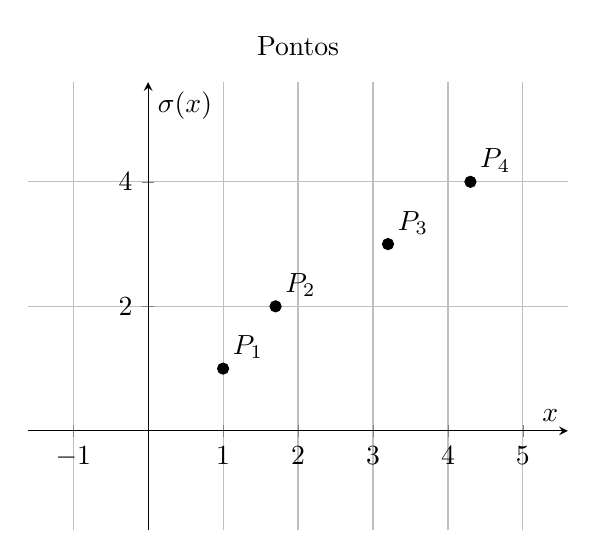
\begin{tikzpicture}
        \begin{axis}[
            title={Pontos},
            xlabel={$x$},
            ylabel={$\sigma(x)$},
            xmin=-1, xmax=5,
            ymin=-1, ymax=5,
            axis lines=middle,
            grid=major,
            enlarge x limits=0.1, 
            enlarge y limits=0.1,
        ]
        \addplot[
            only marks,                     
            mark=*,                       
            mark size=2pt,              
            nodes near coords,             
            point meta=explicit symbolic,   
            nodes near coords align={above right}, 
        ] table [meta=label] { 
            x y label
            1 1 $P_1$
            1.7 2 $P_2$
            3.2 3 $P_3$
            4.3 4 $P_4$ 
        };
        \end{axis}
    \end{tikzpicture}
    \caption{Conjunto de pontos dispostos no plano cartesiano.}%
    \label{fig: pontos_addplot}
    \fonte{O autor (2025).}
\end{figure}

Existe uma técnica que permite que nos façamos isso, ela se chama regressão linear (a qual é um dos tópicos discutidos no Capítulo~\ref{cap:regressao}), e com base nela, é possível dado um conjunto de pontos em um plano, traçar uma reta que se aproxime igualmente de cada um desses pontos. Existem diferentes técnicas de regressão linear, neste caso aplicaremos a dos mínimos quadrados e encontramos a expressão:

\[ y=0.8623x+0.3011 \]

Com base nessa função que encontramos, podemos desenhá-la junto ao gráfico dos pontos e vermos se ela é realmente uma boa aproximação, assim temos a Figura~\ref{fig: regressao-linear}

\begin{figure}[h!]
    \centering
    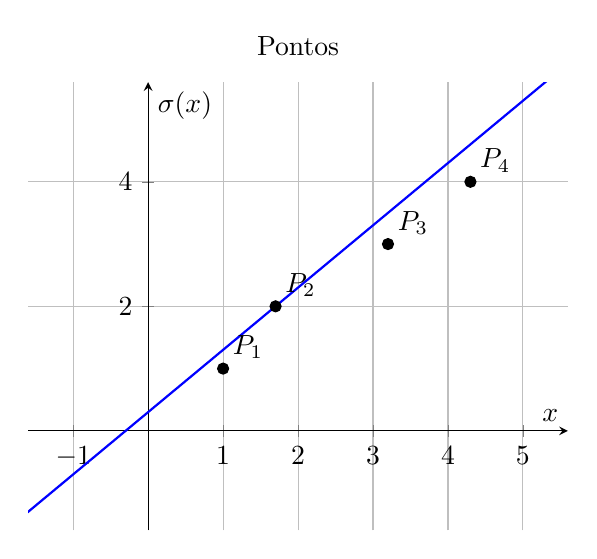
\begin{tikzpicture}
        \begin{axis}[
            title={Pontos},
            xlabel={$x$},
            ylabel={$\sigma(x)$},
            xmin=-1, xmax=5,
            ymin=-1, ymax=5,
            axis lines=middle,
            grid=major,
            enlarge x limits=0.1, 
            enlarge y limits=0.1,
        ]
        \addplot[
            only marks,                     
            mark=*,                       
            mark size=2pt,              
            nodes near coords,             
            point meta=explicit symbolic,   
            nodes near coords align={above right}, 
        ] table [meta=label] { 
            x y label
            1 1 $P_1$
            1.7 2 $P_2$
            3.2 3 $P_3$
            4.3 4 $P_4$ 
        };
        \addplot[blue, thick, domain=-8:8, samples=100] {0.8623(x) + 0.3011};
        \end{axis}
    \end{tikzpicture}
    \caption{Conjunto de pontos dispostos no plano cartesiano.}%
    \label{fig: regressao-linear}
    \fonte{O autor (2025).}
\end{figure}

Existem diversas aproximações além da regressão linear, se quisermos, podemos tentar aproximar esses pontos utilizando uma função quadrática, cúbica ou até mesmo exponencial.

Esse tema parece não ter uma conexão com esse capítulo de funções de ativação, mas na realidade, o que muitas das vezes é feito por uma rede neural é justamente esse trabalho de encontrar uma função que aproxima o comportamento de um conjunto de pontos. Só que neste caso, não teremos um conjunto de pontos, vamos ter várias informações em uma base de dados, como imagens de exames médicos ou informações sobre o valor de imóveis e queremos encontrar de alguma forma uma conexão entre esses dados.

Para isso, existe um conjunto de teoremas que servem justamente para provar que uma determinada rede neural criada será capaz de encontrar uma função que descreva o comportamento que você esteja estudando. Eles são os teoremas da aproximação universal.

No livro \textit{Deep Learning}, \textcite{DeepLearningBook} dedicam uma seção explicando esses teoremas. Segundo os autores, o teorema da aproximação universal, introduzido \textcite{Cybenko1989} para a comunidade científica no texto \textit{Approximation by Superpositions of a Sigmoidal Function}, afirma que uma rede \textit{feedforward} com uma camada de saída linear e no mínimo uma camada oculta com qualquer função que possui a propriedade de ``esmagamento'', como a sigmoide logística, é capaz de aproximar qualquer função mensurável de Borel de um espaço de dimensão finita para outro com qualquer quantidade de erro diferente de zero desejada desde que essa rede neural possua unidades ocultas suficientes.

Para entendermos esse teorema, devemos primeiro entender o conceito de mensurabilidade de Borel, segundo \textcite{DeepLearningBook} uma função contínua em um subconjunto fechado e limitado de $\mathbb{R}^N$ é mensurável por Borel. Assim esse tipo de função pode ser aproximada por uma rede neural. Além disso, os autores ressaltam que por mais que o teorema original tenha conseguido provar apenas para as funções que saturam tanto para termos muito negativos ou termos muito positivos, diversos outros autores como \textcite{Leshno1993}, no texto \textit{Multilayer feedforward networks with a nonpolynomial activation function can approximate any function}, foram capazes de provar que o teorema da aproximação universal pode funcionar para outras funções, no caso de Leshno, eles provaram para funções não polinomiais, como a \textit{Rectified Linear Unit} (\textit{ReLU}), a qual é o tema central do Capítulo~\ref{cap:ativacao-retificadoras}.

Basicamente os teoremas da aproximação universal reforçam o uso de funções de ativação para permitir que as redes neurais resolvam os problemas propostos por meio da aproximação de uma função. Isso acontece porque essas funções introduzem a não-linearidade para a rede, como nos vimos na equação do neurônio de uma rede neural, uma rede neural é composta por diferentes camadas de neurônios que são capazes de pegar valores de entrada, multiplicar por um peso dado e somar com um viés, esse resultado passa então por uma função de ativação.

\[ x_j = (\sum_i y_i \cdot w_{ji}) + b_j \]

Se nos tivéssemos uma rede neural em que os neurônios não possuíssem uma função de ativação, ou, fosse uma função linear, mesmo juntando todas essas camadas de neurônios que trazem expressões lineares, a junção disso, ainda seria uma expressão linear. Mas quando introduzimos uma função não linear, como a sigmoide, o teorema da aproximação universal, nos garante que somos capazes de encontrar qualquer função que estivermos procurando, desde que ela seja mensurável de Borel.

\section{Propriedades das Funções de Ativação: Escolhendo Uma Boa Função de Ativação}%
\index{Propriedades das funções de ativação}

Visto um dos motivos de se utilizar funções de ativação em uma rede neural, cabe agora entender um pouco dessa classe de funções. Em \textit{A Survey on Activation Functions and their relation with Xavier and He Normal Initialization}, \textcite{PropriedadesFuncoesDeAtivacao} discute algumas das propriedades das funções de ativação, dizendo que é esperado que essas funções sejam: não-lineares, diferenciáveis, contínuas, limitadas, centradas em zero. Além disso, o autor discute também que é interessante considerar também o custo computacional dessas funções que estão sendo aplicadas em uma rede neural \parencite{PropriedadesFuncoesDeAtivacao}.

Dessa forma, é possível discutir elaborar pouco de cada uma dessas propriedades em seguida.

\medskip
\textbf{Não-linearidade}
\medskip

Como foi visto na seção anterior, o principal objetivo de uma função de ativação ser não linear é justamente relacionado ao fato delas permitirem que um modelo seja capaz de aproximar diversos tipos de funções desde que sejam mensuradas por Borel. Além disso, \textcite{PropriedadesFuncoesDeAtivacao} justifica que caso tenha uma rede como um \textit{Perceptron} com múltiplas camadas ocultadas pode ser facilmente comprimido em um \textit{perceptron} de apenas uma camada. Isso acontece porque a várias transformações lineares (uma para cada camada) em cima de outras também lineares continuam formando uma transformação linear quando serem consideradas por inteiro. Com isso, o principal benefício de uma rede neural, que é a profundidade, acaba por não ter tanto efeito em casos em que são aplicadas funções de ativação lineares.

\medskip
\textbf{Diferenciabilidade}
\medskip

O principal motivo de considerar a diferenciabilidade ao se escolher uma função de ativação está intrinsecamente ligado em como a retropropagação do erro. Como visto no Capítulo~\ref{cap:retropropagacao-gradiente}, a retropropagação utiliza das derivadas parciais, do vetor gradiente e também da derivada da função de ativação para calcular o erro e com base neste, as atualizações dos pesos e vieses da rede. Perceba que escolher uma função que tenha uma derivada complexa ou não seja derivada em grande parte do seu domínio, acaba por atrasar o algoritmo da retropropagação, que levará mais tempo tendo que calcular a derivada da função de ativação ou terão que ser feitas adaptações na derivada da função original para adequá-la ao novo algoritmo.

\medskip
\textbf{Continuidade}
\medskip

A continuidade está ligada com a diferenciabilidade. Pela definição de derivada, não é possível derivar uma função em pontos de descontinuidade. Dessa forma, é importante considerar como o a função é representada graficamente, garantindo que não haja ``quinas'' no desenho da função e que o gráfico pode ser desenhado ``sem tirar o lápis do papel''. Técnicas como essas ajudam a descobrir ao olhar o gráfico, se existem pontos de descontinuidade os quais podem afetar a derivada da função de ativação.

\medskip
\textbf{Limitada}
\medskip

Considerar que uma função de ativação seja limitada ao escolher uma função de ativação para construir uma rede neural está ligado com os problemas do gradiente. Neste caso, uma função que não é limitada pode sofrer do problema do gradiente explosivo, o qual é explicado com maiores detalhes no Capítulo~\ref{cap:ativacao-retificadoras}. Nesse sentido, o problema do gradiente explosivo o gradiente de uma rede neural começa a crescer de forma acelerada afetando o aprendizado da rede e as atualizações de pesos e vieses.

\medskip
\textbf{Centrada em zero}
\medskip

Uma função que não é centrada em zero, que é sempre positiva ou sempre negativa, afeta como a saída ocorre \parencite{PropriedadesFuncoesDeAtivacao}. Como explica \textcite{PropriedadesFuncoesDeAtivacao}, um cenário em que isso acontece, significa que a saída está sendo sempre movida para os valores positivos ou negativos, e como resultado, o vetor de pesos precisa de uma quantidade maior de iterações para ser melhor ajustado. Dessa forma, ao escolher uma função que é centrada em zero, é possível garantir um treinamento com menos iterações mas ainda assim garantir uma boa convergência do modelo que está sendo treinado.

\medskip
\textbf{Custo computacional}
\medskip

Cabe considerar também o custo computacional de uma função de ativação. Funções mais simples, como a degrau unitário e a \textit{ReLU}, as quais fazem apenas comparações com o valor da entrada, apresentam um custo computacional bem menor quando comparadas com funções mais complexas, como aquelas que fazem uso de muitos exponenciais em sua fórmula. Com isso, ao utilizar uma função de ativação muito ``cara'' em termos computacionais, isso acaba por gerar um gargalo no tempo de treino do modelo em desenvolvimento.

\medskip
\begin{center}
 * * *
\end{center}
\medskip

Vale destacar também que muitas dessas propriedades não estão presentes em todas as funções de ativação. A sigmoide por exemplo é uma função que não está centrada em zero, possuindo apenas saídas positivas. Já a \textit{ReLU} apresenta um ponto de descontinuidade na origem, mas isso não atrapalha essas funções de ativação de serem utilizadas ao construir uma rede neural. As propriedades servem mais como um guia, destacando vantagens que se pode ter ao utilizar determinada função de ativação.

Considerando isso, é possível finalmente entrar no tópico principal desse capítulo: as funções sigmoidais. Para isso, será explicado antes um exemplo ilustrativo destacando como essas funções atuam ao receberem suas entradas.

\section{Exemplo Ilustrativo: Empurrando para Extremos}

Imagine que você está trabalhando para uma empresa na área de marketing e precisa analisar como foi a recepção do público para um novo produto anunciado. Para isso, você ficou responsável por classificar os comentários do público sobre esse produto. Você precisa colocar eles em duas categorias: avaliação positiva ou negativa. Então você precisa ler cada comentário e colocar ele em uma dessas categorias. 

No começo foi fácil, mas depois de um tempo foi ficando repetitivo, então você teve a ideia de automatizar esse processo. Assim, você decide criar um diagrama de uma ``caixa-preta'' responsável por classificar automaticamente esses comentários da mesma forma que estava fazendo. Essa “caixa” irá receber uma entrada, neste caso, o texto do comentário sobre o produto, e irá retornar uma saída, uma classificação positiva ou negativa sobre o comentário. 

Na matemática, as funções do tipo sigmoide são excelentes para esse tipo de problema, pois possuem uma propriedade muito interessante: dado um valor de entrada, elas são capazes de ``empurrar'' esse valor para dois diferentes extremos. No caso da sigmoide logística, a função que dá nome a essa família, ela é capaz de empurrar essa entrada para valores próximos de zero ou um. Se nós consideramos que zero é uma avaliação negativa e um é uma avaliação positiva, essa função se torna perfeita para resolver o seu problema de classificar comentários.

\section{A Sigmoide Logística: Ótima para Classificações Binárias}%
\index{Funções de Ativação!Sigmoide Logística}

Por mais que a \gls{sigmoide} hoje em dia seja bem comum em redes neurais, seu uso não começou nesse cenário. A sigmoide tem suas origens a analise de crescimento populacional e demografia, ela nao surgiu em um artigo em especifico, sendo mais uma evolução presente em vários artigos do matemático belga Pierre François Verhulst dentre os anos de 1838 e 1847. Contudo, existe um artigo desse matemático, intitulado \textit{Recherches mathématiques sur la loi d'accroissement de la population} (Pesquisas matemáticas sobre a lei de crescimento da população), em que \textcite{SigmoidVerhulst1845} propõe a função logística como um modelo para descrever o crescimento populacional, levando em consideração a capacidade de suporte de um ambiente, isso gerou a curva em ``S'' característica da sigmoide. Contudo, foi somente no próximo século, que sigmoide passou a ser utilizada na area da ciência da computação.

Nos anos 1980, estavam ocorrendo mudanças com as funções que eram utilizadas para construir uma rede neural, um desses motivos foi a introdução da retropropagação pelos pesquisadores David Rumelhart, Geoffrey Hinton e Ronald Williams. A retropropagação era uma técnica que permitia que um modelo aprendesse com base nos seus erros, ajustando automaticamente os seus parâmetros em busca de conseguir uma melhor acurácia \parencite{BackpropagationArticle}. 

Além disso, na pesquisa que introduz a retropropagação, \textit{Learning representations by back-propagating errors} de 1986, os cientistas propõem o uso da função sigmoide logística como uma das candidatas para ser utilizada junto com a retropropagação como uma função de ativação, como justificativa, \textcite{BackpropagationArticle} citam o fato dela ser uma função que é capaz de introduzir a não-linearidade para o modelo, permitindo que ele aprenda padrões mais complexos, e também por possui uma derivada limitada.

Mas esse não foi o único fator que fez com que a sigmoide e sua familia se tornassem funções populares para a época. Pouco antes da criação da retropropagação, na década passada, haviam cientistas estudando o comportamento dos neurônios humanos como inspiração para a criação de redes neurais artificiais. Um exemplo desse caso foi o dos cientistas \textcite{SigmoidWilsonCowan}, no início dos anos 70 eles publicaram um artigo intitulado \textit{excitatory and Inhibitory interactions in localized populations of model neurons}, em que buscam estudar como os neurônios respondiam a determinados estímulos.

No artigo, Hugh e Cowan buscam analisar o comportamento de populações localizadas de neurônios excitatórios (denotados pela função $E(t)$) e inibitórios (representados por $I(t)$) e como as duas interagem entre si, para isso, eles utilizam como variável a proporção de células em uma subpopulação que dispara/reage por unidade de tempo \parencite{SigmoidWilsonCowan}. Para modelar essa atividade, \textcite{SigmoidWilsonCowan} fizeram o uso uma variação da função sigmoide, representada para Equação~\ref{eq:neuronio-de-wilson-cowan}, que era capaz de descrever o comportamento dos neurônios a certos estímulos.

\begin{equacaodestaque}{Neurônio de Wilson e Cowan}
    \mathcal{S}(x) = \frac{1}{1 + e^{-a(x - \theta)}} - \frac{1}{1 + e^{a\theta}}%
    \label{eq:neuronio-de-wilson-cowan}
\end{equacaodestaque}


Nessa equação, o parâmetro $a$ representa a inclinação, a qual foi ajustada para passar pela origem ($\mathcal{S}(0) = 0$) e $\theta$ 
é o limiar. Para o plotar o gráfico da Figura~\ref{fig:sigmoide-wilson-e-cowan}, foi utilizado os mesmos valores escolhidos pelos cientistas na pesquisa, assim $a = 1.2$ e $\theta = 2.8$.

\begin{figure}[h!]

    \pgfmathdeclarefunction{wilson_sigmoid}{3}{% 
        \pgfmathparse{1/(1+exp(-#1*(#3-#2))) - 1/(1+exp(#1*#2))}%
    }

    \centering
    \begin{tikzpicture}
        \begin{axis}[
            title={Função Sigmoide de Wilson-Cowan},
            xlabel={$x$ (Estímulo)},
            ylabel={$s(x)$ (Proporção de Ativação)},
            xmin=-2, xmax=10, % Ajusta o eixo x para centralizar a curva
            ymin=-0.1, ymax=1.1, % Ajusta o eixo y
            axis lines=middle,
            grid=major,
            legend pos=north west,
            % Define os parâmetros para a função
            /pgf/declare function={a=1.2; theta=2.8;}
            ]
            \addplot[blue, thick, domain=-2:10, samples=150] {wilson_sigmoid(a, theta, x)};
        \end{axis}
    \end{tikzpicture}
    \caption{Gráfico da função sigmoide conforme proposta por Wilson e Cowan (1972), com parâmetros de exemplo $a=1.2$ e $\theta=2.8$.}%
    \label{fig:sigmoide-wilson-e-cowan}
\end{figure}

\textcite{SigmoidWilsonCowan} demonstram que a população de neurônios reage de formas distintas quando sofrem determinados estímulos, os níveis baixos de excitação não conseguem ativar a população, porém, existe uma região de alta sensibilidade, na qual pequenos aumentos no estímulo geram um grande aumento na atividade. Além disso, existe um terceiro nível, o de saturação, em que níveis muito altos de estímulos são capazes de ativar todas as células e a partir disso, a resposta da população atinge o comportamento de uma função constante, indicando que ela saturou \parencite{SigmoidWilsonCowan}. Ao juntar todos esses três níveis, tem-se a famosa curva em ``S'', caraterística da função sigmoide.

Com isso, ao consideramos esses dois cenários: a criação da retropropagação e busca na natureza para inspiração na criação de redes neurais. A sigmoide, junto com a sua família, se tornaram funções muito populares para a época, estando presentes em varias redes neurais criadas. Um desses exemplos é a rede de Elman, um tipo de rede neural recorrente criada para aprender e representar estruturas em dados sequenciais, \textcite{ElmanNetwork} cita em seu estudo \textit{Finding structure in time} que era ideal o uso de uma função de ativação com valores limitados entre zero e um. Um cenário perfeito para o uso da sigmoide logística.

Cabe destacar também que, as sigmoidais nao foram as primeiras funções de ativação a serem utilizadas na criação de uma rede neural. Nesse cenário de redes neurais, existem sempre funções que são mais populares, e que com o tempo e o surgimento de novas pesquisas, são deixadas de lado para novas funções mais interessantes. Uma função que era muito utilizada era a \textit{heavside}, ou degrau unitário em português, ela está representada na Figura~\ref{fig:degrau-unitario}. Essa função inclusive esteve presente na produção da rede neural \textit{Perceptron} criada por \textcite{PerceptronRosenblatt} e introduzida para a comunidade científica no artigo \textit{The Perceptron: A probabilistic model for informations storage and organization in the brain} no final dos anos 50.

\begin{figure}[h!]
    \centering
    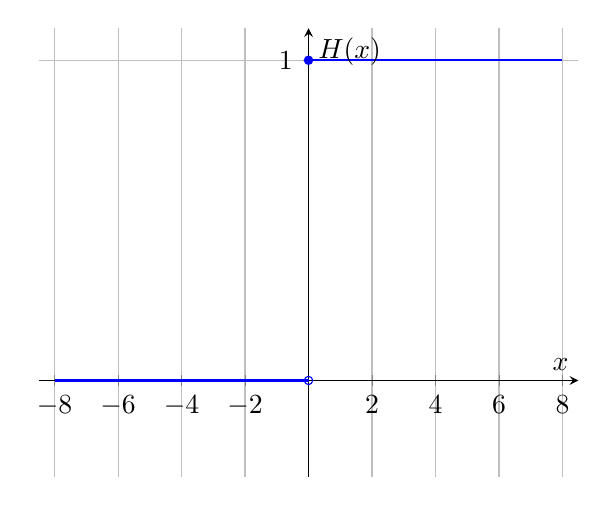
\begin{tikzpicture}
        \begin{axis}[
            xlabel={$x$},
            ylabel={$H(x)$},
            xmin=-8.5, xmax=8.5,
            ymin=-0.3, ymax=1.1,
            axis lines=middle,
            grid=major,
            ytick={0,1}, % Define os ticks no eixo y para 0 e 1
        ]
        % Desenha a parte da função para x < 0
        \addplot[blue, thick, domain=-8:0] {0};
        % Desenha a parte da função para x >= 0
        \addplot[blue, thick, domain=0:8] {1};

        % Adiciona os marcadores para a descontinuidade em x=0
        % Círculo aberto em (0,0) para indicar que o ponto não pertence a essa parte
        \addplot[only marks, mark=o, mark size=1.5pt, blue, fill=white] coordinates {(0,0)};
        % Círculo fechado em (0,1) para indicar que o ponto pertence a essa parte
        \addplot[only marks, mark=*, mark size=1.5pt, blue] coordinates {(0,1)};
        \end{axis}
    \end{tikzpicture}
    \caption{Gráfico da função degrau unitário (\textit{heavside}).}
    \label{fig:degrau-unitario}
    \fonte{O autor (2025).}
\end{figure}

Ao comparar a degrau unitário com a sigmoide, é possível notar uma diferença crucial, a sigmoide é uma função contínua em todos os pontos, podemos dizer que para desenhar seu gráfico não precisamos tirar o lápis do papel nenhuma vez, algo que não ocorre com a \textit{heavside}. Além disso, a derivada da \textit{heavside} é zero em quase todos os seus pontos, por esse motivo, ela impossibilitava a retropropagação do erro, uma vez que quando fossemos calcular o gradiente para uma parte de um modelo que usasse essa função, ele provavelmente seria zero.

A função sigmoide é escrita com uma exponencial, como na Equação~\ref{eq:sigmoide}. Como explica \textcite{ActivationFunctionsLederer}, a sigmoide ela é uma função limitada, diferenciável e monotônica, o que significa que conforme os valores de $x$ aumentam os valores de $f(x)$ também aumentam.

\begin{equacaodestaque}{Sigmoide Logística}
    \sigma(x_j) = \frac{1}{1 + e^{-x_j}}
    \label{eq:sigmoide}
\end{equacaodestaque}

Em que:

\begin{itemize}
    \item $x_j$ representa o valor da entrada da função de ativação
\end{itemize}

O gráfico da sigmoide está presente na Figura~\ref{fig:sigmoide}, note que ele possui o formato de um ``S'' deitado. Assim, também é possível dizer que a função sigmoide é uma função suave, contínua (o que a possibilita de ser derivável em todos os pontos) e também é não-linear. \textcite{ActivationFunctionsLederer} explica que uma das propriedades interessantes da sigmoide está no fato dela empurrar os valores de entrada para dois extremos, neste caso, 0 e 1. Essa propriedade de retornar valores em um intervalo de 0 a 1 é bem útil quando queremos fazer uma classificação binária, para isso, utilizamos a sigmoide aplicada na última camada densa de neurônios, limitando os intervalos, de forma que podemos interpretá-los como probabilidades, em que quanto mais próximo de 1, mais próximo aquele resultado está de uma classe A, por exemplo, já valores mais distantes pertenceriam a uma classe B.

\begin{figure}[h!]
    \centering
    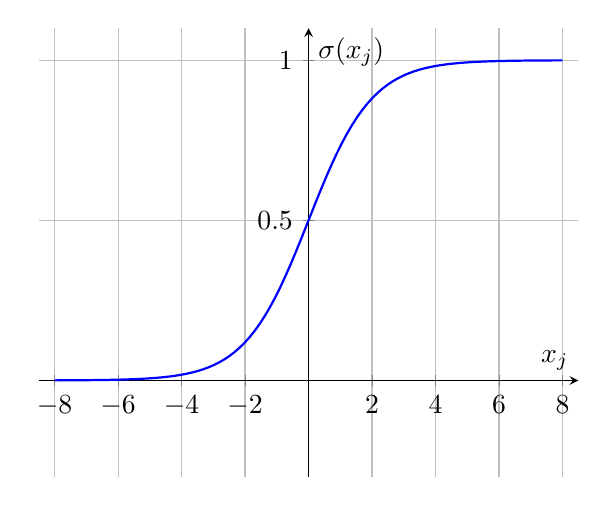
\begin{tikzpicture}
        \begin{axis}[
            xlabel={$x_j$},
            ylabel={$\sigma(x_j)$},
            xmin=-8.5, xmax=8.5,
            ymin=-0.3, ymax=1.1,
            axis lines=middle,
            grid=major,
        ]
        \addplot[blue, thick, domain=-8:8, samples=100] {1/(1+exp(-x))};
    \end{axis}
    \end{tikzpicture}
    \caption{Gráfico da função de ativação sigmoide logística.}%
    \label{fig:sigmoide}
    \fonte{O autor (2025).}
\end{figure}

\medskip
\begin{center}
 * * *
\end{center}
\medskip

\textbf{Características da Sigmoide Logística}
\vspace{1em}

\begin{itemize}
    \item \textbf{Continuidade, suavidade e diferenciabilidade:}
    \item \textbf{Não-linearidade:}
    \item \textbf{Limitada:}
    \item \textbf{Saturante:}
\end{itemize}

\medskip
\begin{center}
 * * *
\end{center}
\medskip

Um ponto a ser destacado nas funções de ativação, e que começou a ser visto no capítulo anterior (Capítulo~\ref{cap:retropropagacao-gradiente}), é que se estamos construindo um modelo que aprende por meio da retropropagação, nós estamos também interessados em entender como essas funções de ativação se comportam em suas derivadas, pois ela é um dos componentes básicos para se calcular o gradiente retropropagado.

Assim, ao derivar a sigmoide logística é possível encontrar a Equação~\ref{eq:sigmoide-derivada}.

\begin{equacaodestaque}{Sigmoide Logística Derivada}
    \frac{d}{dx_j}[\sigma](x_j) = \frac{e^{-x_j}}{(1 + e^{-x_j})^2}%
    \label{eq:sigmoide-derivada}
\end{equacaodestaque}

Um ponto a ser destacado é que a sigmoide também pode ser expressa de uma forma recursiva, algo que é muito útil pois ajuda a poupar cálculos a serem feitos. Dessa forma, também tem-se a Equação~\ref{eq:sigmoide-derivada-recursiva}.

\begin{equacaodestaque}{Sigmoide Logística Derivada Recursivamente}
    \frac{d}{dx_j}[\sigma](x_j) = \sigma(x_j)(1 - \sigma(x_j))%
    \label{eq:sigmoide-derivada-recursiva}
\end{equacaodestaque}

Tendo a sua derivada, cabe também plotar o seu gráfico para ver o seu comportamento. Com isso, a derivada da sigmoide logística pode ser vista na Figura~\ref{fig:sigmoide-derivada}. Perceba que o valor máximo que a derivada da sigmoide retorna é pouco maior que 0.2, esse é um dos pontos que mais atrapalha as redes que fazem uso de muitas funções sigmoidais, porque acaba por gerar um problema conhecido por desaparecimento do gradiente. Mas é importante destacar o quão importante são as derivadas das funções de ativação, pois muitas vezes elas acabam por gerar diversos problemas.

\begin{figure}[h!]
    \centering
    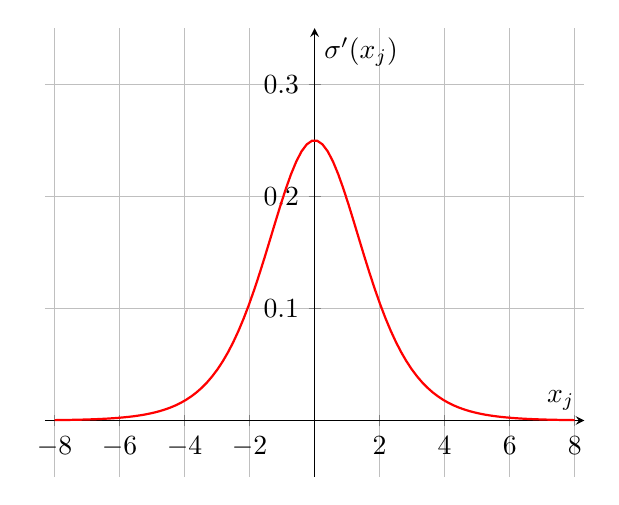
\begin{tikzpicture}
        \begin{axis}[
            xlabel={$x_j$},
            ylabel={$\sigma'(x_j)$},
            xmin=-8.3, xmax=8.3,
            ymin=-0.05, ymax=0.35,
            axis lines=middle,
            grid=major,
        ]
        \addplot[red, thick, domain=-8:8, samples=100] {exp(-x)/((1+exp(-x))^2)};
        \end{axis}
    \end{tikzpicture}
    \caption{Gráfico da derivada da função de ativação sigmoide logística.}%
    \label{fig:sigmoide-derivada}
    \fonte{O autor (2025).}
\end{figure}

\medskip
\begin{center}
 * * *
\end{center}
\medskip

\textbf{Algumas Aplicações da Sigmoide Logística em Redes Neurais}%
\index{Aplicações práticas! Sigmoide logística}
\vspace{1em}

\begin{itemize}
    \item \textbf{Aplicação 1 (Área):}
    \item \textbf{Aplicação 2 (Área):}
    \item \textbf{Aplicação 3 (Área):}
    \item \textbf{Aplicação 4 (Área):}
\end{itemize}

\medskip
\begin{center}
 * * *
\end{center}
\medskip

Conhecendo a sigmoide logística, a função que dá nome a essa família de funções de ativação, é possível conhecer agora outras funções dessa mesma família. Essas funções apresentam propriedades semelhantes com a sigmoide, como a característica curva em ``S'' mas com algumas variações em sua estrutura ou fórmula, as quais podem ser úteis em alguns cenários.

Para isso, será vista primeira a tangente hiperbólica, e como ela melhora uma das desvantagens da sigmoide, com o fato dessa nova função ser centrada em zero.

\section{Tangente Hiperbólica: A Pioneira nas Redes Convolucionais}%
\index{Funções de Ativação!Tangente Hiperbólica (tanh)}

Assim como a função sigmoide, a \gls{tangente-hiperbolica} não possui suas origens voltadas para o uso em redes neurais. Neste caso, um dos matemáticos que ficou reconhecido por criar a notação das funções hiperbólicas, seno, cosseno e tangente, foi o suíço Johann Heinrich Lambert no trabalho de 1769 \textit{Mémoire sur quelques propriétés remarquables des quantités transcendantes circulaires et logarithmiques} (Memória sobre algumas propriedades notáveis de grandezas transcendentais circulares e logarítmicas), em que provou que muitas das identidades trigonométricas possuíam suas equivalentes hiperbólicas \parencite{TanhLambert}.

Passado mais de dois séculos, a tangente hiperbólica já estava sendo utilizada em diversas redes neurais, ela inclusive fez parte da primeira rede neural convolucional criada, estando presente na \textit{Le-Net-5}, uma rede neural criada para identificar e classificar imagens de cheques em caixas eletrônicos \parencite{LecunLeNet1998}. No artigo acadêmico \textit{Gradient-based learning applied to document recognition} de 1998, os cientistas \textcite{LecunLeNet1998} explicam a criação dessa rede além de destacar suas métricas alcançadas.

É possível escrever a tangente hiperbólica utilizando a definição de tangente, que é o quociente a função seno com a função cosseno, só que neste caso usando as funções hiperbólicas. Assim ela é representada pela Equação~\ref{eq:tanh}.

\begin{equacaodestaque}{Tangente Hiperbólica (tanh)}
    \mathcal{A}_{\tanh(x_j)} = \frac{\sinh(x_j)}{\cosh(x_j)} = \frac{e^x_j - e^{-x_j}}{e^x_j + e^{-x_j}}%
    \label{eq:tanh}
\end{equacaodestaque}

Em que:

\begin{itemize}
    \item $x_j$ representa o valor da entrada da função de ativação
\end{itemize}

Semelhante a sigmoide, a tangente hiperbólica possui várias propriedades parecidas. Como afirma \textcite{ActivationFunctionsLederer}, a tangente hiperbólica é infinitamente diferenciável, sendo uma versão escalada e rotacionada da sigmoide logística. Assim, veja no gráfico da Figura~\ref{fig:tanh} que ela é uma função que está centrada em zero, e seus valores variam agora em um intervalo de -1 a 1, diferente da sigmoide, que varia somente de 0 a 1.

\begin{figure}[h!]
    \centering
    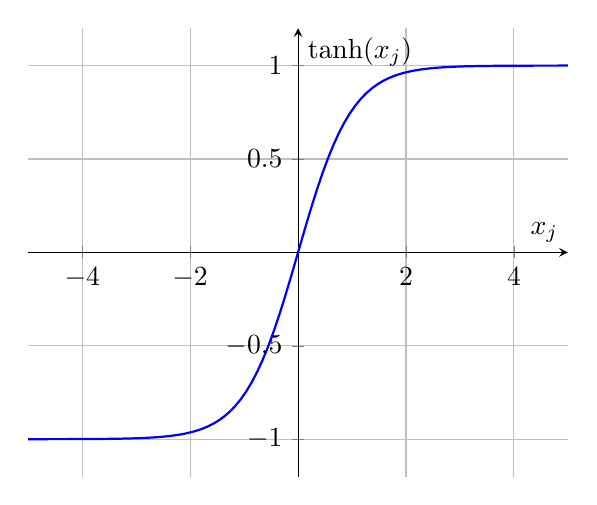
\begin{tikzpicture}
        \begin{axis}[
            xlabel={$x_j$},
            ylabel={$\tanh(x_j)$},
            xmin=-5, xmax=5,
            ymin=-1.2, ymax=1.2,
            axis lines=middle,
            grid=major,
        ]
        \addplot[blue, thick, domain=-5:5, samples=100] {tanh(x)};
        \end{axis}
    \end{tikzpicture}
    \caption{Gráfico da função de ativação tangente hiperbólica (tanh).}%
    \label{fig:tanh}
    \fonte{O autor (2025).}
\end{figure}

\medskip
\begin{center}
 * * *
\end{center}
\medskip

\textbf{Características da Tangente Hiperbólica}
\vspace{1em}

\begin{itemize}
    \item \textbf{Continuidade, suavidade e diferenciabilidade:}
    \item \textbf{Não-linearidade:}
    \item \textbf{Limitada:}
    \item \textbf{Saturante:}
    \item \textbf{Centrada em zero:}
\end{itemize}

\medskip
\begin{center}
 * * *
\end{center}
\medskip

Como foi visto em seções anteriores, é interessante ao escolher uma função de ativação verificar se ela é centrada em zero, como no caso da tangente hiperbólica. Isso acontece pois funções desse tipo permitem uma convergência mais rápida do modelo para os pontos de mínimo, garantindo um melhor desempenho com menos iterações, quando comparadas com funções que não são centradas em zero, como a sigmoide.

De forma análoga a feita na sigmoide logística, vale a pena calcular a derivada da tangente hiperbólica para entender como o gradiente é propagado para as camadas anteriores ao utilizar essa função de ativação. Dessa forma, a sua derivada está representada na Equação~\ref{eq:tanh-derivada}.

\begin{equacaodestaque}{Tangente Hiperbólica (tanh) Derivada}
    \frac{d}{dx_j}[\mathcal{A}_{\tanh}](x_j) = \text{sech}^2(x_j)%
    \label{eq:tanh-derivada}
\end{equacaodestaque}

Assim como a sigmoide logística, a tangente hiperbólica possui uma vantagem, ela pode ser escrita de forma recursiva, o que ajuda a poupar cálculos para a o \textit{backward pass}, pois é possível simplesmente armazenar o resultado dessa função que estava calculado no \textit{forward pass} e reutilizá-lo ao calcular a sua derivada. Isso é muito útil pois quanto menos cálculos forem feitos, maior é a tendência que o modelo será mais rápido e com isso irá convergir em menos tempo\footnote{Note que tanto a sigmoide quanto a tangente hiperbólica fazem uso de exponenciais em suas fórmulas, essas operações acabam por ser caras (em termos de poder de processamento) quando comparadas com as simples operações de comparação da hard tanh, a qual será vista em seções futuras.}. Dessa forma, tem-se que a derivada da tangente hiperbólica escrita de forma recursiva pode ser expressa pela Equação~\ref{eq:tanh-derivada-recursiva}

\begin{equacaodestaque}{Tangente Hiperbólica (tanh) Derivada Recursivamente}
    \frac{d}{dx_j}[\mathcal{A}_{\tanh}](x_j) = 1 - \tanh^2(x_j)%
    \label{eq:tanh-derivada-recursiva}
\end{equacaodestaque}

Tendo as equações da derivada da tangente hiperbólica, o próximo passo é plotar também o seu gráfico, o qual está presenta na Figura~\ref{fig:tanh-derivada}. Note mais uma vez que a tangente hiperbólica possui o mesmo problema que a sigmoide, os valores máximos que ela retorna para a derivada são muito pequenos, esse é um fator recorrente nas funções sigmoidais.

\begin{figure}[h!]
    \centering
    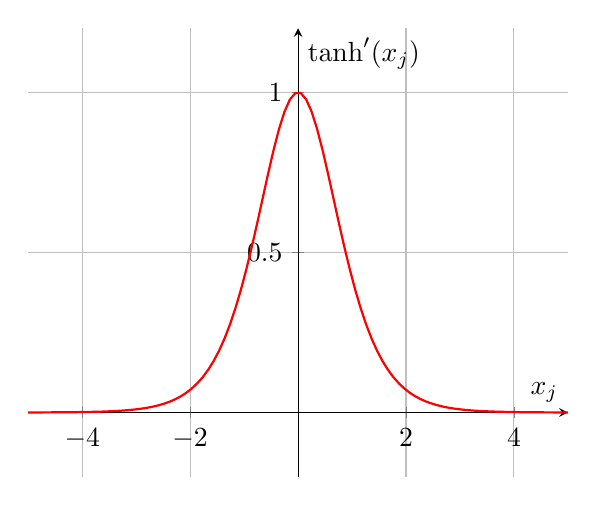
\begin{tikzpicture}
        \begin{axis}[
            xlabel={$x_j$},
            ylabel={$\tanh'(x_j)$},
            xmin=-5, xmax=5,
            ymin=-0.2, ymax=1.2,
            axis lines=middle,
            grid=major,
        ]
        \addplot[red, thick, domain=-5:5, samples=100] {1-(tanh(x))^2};
        \end{axis}
    \end{tikzpicture}
    \caption{Gráfico da derivada da função de ativação tangente hiperbólica (tanh).}%
    \label{fig:tanh-derivada}
    \fonte{O autor (2025).}
\end{figure}

Semelhante a sigmoide, os valores da tangente hiperbólica também se aproximam de zero conforme aumentam ou diminuem na sua derivada. Eles atingem um pico de 1, e conforme as entradas se aproximam de $\pm 4$ a saída da derivada da tangente hiperbólica também fica próxima de zero. Mais uma vez, nota-se que a tangente hiperbólica não atinge valores muito altos em sua derivada, isso acaba por gerar um problema conhecido como desaparecimento do gradiente, o qual será explicado em seções futuras.

\medskip
\begin{center}
 * * *
\end{center}
\medskip

\textbf{Algumas Aplicações da Tangente Hiperbólica em Redes Neurais}%
\index{Aplicações práticas! Tangente hiperbólica (tanh)}
\vspace{1em}

\begin{itemize}
    \item \textbf{Aplicação 1 (Área):}
    \item \textbf{Aplicação 2 (Área):}
    \item \textbf{Aplicação 3 (Área):}
    \item \textbf{Aplicação 4 (Área):}
\end{itemize}

\medskip
\begin{center}
 * * *
\end{center}
\medskip

Por fim, perceba que a tanto a tangente hiperbólica quando a sigmoide logística são funções de ativação ``caras'', por utilizarem exponenciais em sua composição. Assim, a próxima função a ser vista busca justamente corrigir esse problema, possuindo a mesma proposta das sigmoidais, porém, sendo mais ``barata'' em termos de custo computacional.

\section{Softsign: Uma Sigmoidal Mais Barata}%
\index{Funções de Ativação!Softsign}

A próxima função sigmoidal a ser analisada é a \textit{softsign}, diferente da tangente hiperbólica e da sigmoide que tiveram suas origens em outros campos diferentes da ciência da computação, a \textit{softsign} foi criada com o intuito de ser trabalhada em uma rede neural. Ela foi introduzida no artigo \textit{A Better Activation Function for Artificial Neural Networks} de 1993, do cientista \textcite{Softsign1998}, no texto o autor propõe a \textit{softsign} como uma alternativa para as funções sigmoidais tradicionais.

A principal diferença da \textit{softsign} com as outras sigmoidais está na sua fórmula, como pode ser visto na Equação~\ref{eq:softsign} é que ela não utiliza nenhum exponencial para compor sua função. Isso faz com que ela seja uma função mais ``barata'' em termos de custo computacional para ser implementada em redes neurais. Assim, é possível obter resultados parecidos porem utilizando cálculos menos complexos e com isso encontrar redes mais rápidas de serem treinadas.

\begin{equacaodestaque}{\textit{Softsign}}
    \mathcal{A}_{\text{Softsign}}(x_j) = \frac{x_j}{1 + |x_j|}%
    \label{eq:softsign}
\end{equacaodestaque}

Em que:

\begin{itemize}
    \item $x_j$ representa o valor da entrada da função de ativação
\end{itemize}

A \textit{softsign} também possui uma representação gráfica, como vista na Figura~\ref{fig:softsign}, ela possui o formato em ``S'' característico das sigmoidais além de ser centrada em zero como a tangente hiperbólica. Além disso, como \textcite{Softsign1998} destaca em seu texto, ela é uma função que é diferenciável em toda a reta possuindo também a mesma propriedade das outras sigmoidais de empurrar os valores de entrada para os seus extremos. Nota-se também pelo seu gráfico que ela também uma função contínua, suave e não-linear.

\begin{figure}[h!]
    \centering
    % Gráfico da função Softsign usando PGFPlots
    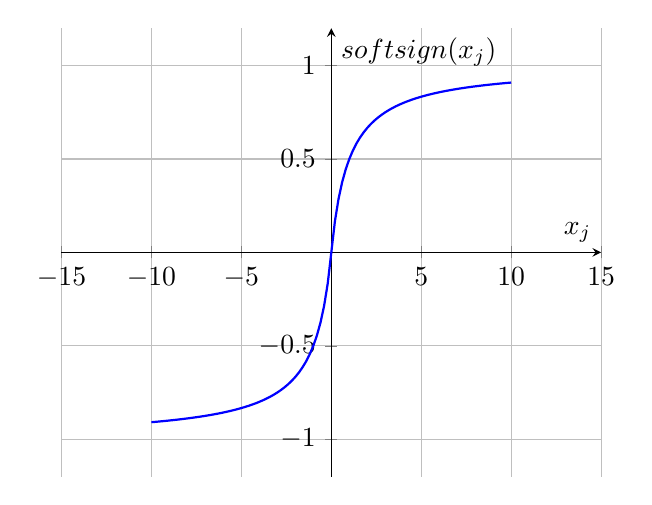
\begin{tikzpicture}
        \begin{axis}[
            xlabel={$x_j$},
            ylabel={$\text{softsign}(x_j)$},
            xmin=-15, xmax=15,
            ymin=-1.2, ymax=1.2,
            axis lines=middle,
            grid=major,
        ]
        % A função softsign(x) = x / (1 + abs(x))
        \addplot[blue, thick, domain=-10:10, samples=101] {x / (1 + abs(x))};
        \end{axis}
    \end{tikzpicture}
    \caption{Gráfico da função de ativação \textit{softsign}.}
    \label{fig:softsign}
    \fonte{O autor (2025).}
\end{figure}

\medskip
\begin{center}
 * * *
\end{center}
\medskip

\textbf{Características da Softsign}
\vspace{1em}

\begin{itemize}
    \item \textbf{Continuidade, suavidade e diferenciabilidade:}
    \item \textbf{Não-linearidade:}
    \item \textbf{Limitada:}
    \item \textbf{Saturante:}
    \item \textbf{Centrada em zero:}
\end{itemize}

\medskip
\begin{center}
 * * *
\end{center}
\medskip

Com relação a sua diferenciabilidade, a \textit{softsign} pode ser derivada em todos os seus pontos, e sua derivada pode ser vista na Equação~\ref{eq:softsign-derivada}. Com base nela, é possível notar uma outra diferença da \textit{softsign} com a tangente hiperbólica e a sigmoide. Diferente das outras duas, a derivada da \textit{softsign} não pode ser expressa em termos da sua própria função. Assim, enquanto nas outras funções é feito um cálculo complexo na função e um simples na derivada, pois é aproveitado o resultado, na \textit{softsign} isso não ocorre.

\begin{equacaodestaque}{\textit{Softsign} Derivada}
    \frac{d}{dx_j}[\mathcal{A}_{\text{softsign}}](x_j) = \frac{1}{(1 + |x_j|)^2}%
    \label{eq:softsign-derivada}
\end{equacaodestaque}

Tendo a sua derivada, cabe também plotar o gráfico da derivada da \textit{softsign}, apresentado na Figura~\ref{fig:softsign-derivada}. Perceba que o valor de sua derivada começa a ficar proximo de zero quando $x$ se aproxima de $\pm 10$, indicando que ela começa a saturar nesse ponto. Com isso, nota-se que ela demora mais para saturar quando comparada com as outras sigmoidais vistas até o momento.

\begin{figure}[h!]
    \centering
    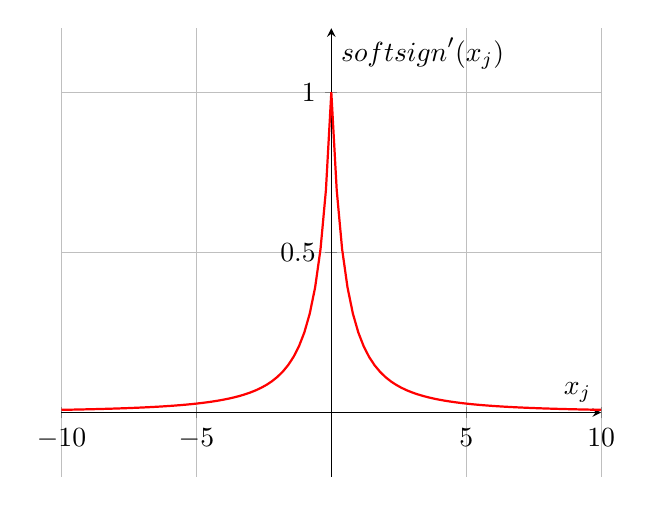
\begin{tikzpicture}
        \begin{axis}[
            xlabel={$x_j$},
            ylabel={$\text{softsign}'(x_j)$},
            xmin=-10, xmax=10,
            ymin=-0.2, ymax=1.2,
            axis lines=middle,
            grid=major,
        ]
        % A derivada da softsign é 1 / (1 + |x|)^2
        \addplot[red, thick, domain=-10:10, samples=101] {1/((1+abs(x))^2)};
        \end{axis}
    \end{tikzpicture}
    \caption{Gráfico da derivada da função de ativação \textit{softsign}.}%
    \label{fig:softsign-derivada}
    \fonte{O autor (2025).}
\end{figure}

Além disso, essa função também sofre do mesmo problema das outras duas funções de ativação vistas até agora, o problema do desaparecimento do gradiente. Esse é um ponto que é corrigido com uma outra família de funções de ativação, as retificadoras, as quais são tema principal do Capítulo~\ref{cap:ativacao-retificadoras}.

\medskip
\begin{center}
 * * *
\end{center}
\medskip

\textbf{Algumas Aplicações da Softsign em Redes Neurais}%
\index{Aplicações práticas! Softsign}
\vspace{1em}

\begin{itemize}
    \item \textbf{Aplicação 1 (Área):}
    \item \textbf{Aplicação 2 (Área):}
    \item \textbf{Aplicação 3 (Área):}
    \item \textbf{Aplicação 4 (Área):}
\end{itemize}

\medskip
\begin{center}
 * * *
\end{center}
\medskip

Seguindo na proposta de ver funções sigmoidais que são mais ``baratas'', a próxima seção busca explorar isso com outras duas funções: a \textit{hard sigmoid} e a \textit{hard tanh}. Essas funções tem como intuito imitar o comportamento das sigmoidais porém, escrito em forma de retas, dessa forma, elas sacrificam a suavidade das sigmoidais para garantir um menor custo computacional.

\section{Hard Sigmoid e Hard Tanh: O Sacrifício da Suavidade em Prol do Desempenho}%
\index{Funções de Ativação!Hard Sigmoid}%
\index{Funções de Ativação!Hard Tanh}

Agora será visto duas funções sigmoidais, criadas no contexto de redes neurais, cujo o seu intuito é ser trazer velocidade para o modelo que está sendo criado, elas são a \gls{hard-sigmoid} e \gls{hard-tanh}. Elas são inspiradas nas suas versões originais ou \textit{soft}, com o mesmo intuito de variar até um certo ponto e depois saturar. Contudo, não garantem a mesma suavidade que as outras funções.

A primeira é a \textit{hard sigmoid}. Como pode ser visto na Equação~\ref{eq:hard-sigmoid}, a qual está presente na documentação do \textcite{PyTorchHardSigmoid}, ela pode ser escrita juntando 3 diferentes funções, duas delas sendo funções constantes e uma terceira sendo a função identidade. Note que ela perde a suavidade da função seno, possuindo bicos que a impedem de ser derivada em todos os seus pontos, contudo, seus cálculos são bem mais simples quando comparados com a sigmoide tradicional, não tem nenhuma exponencial para atrasar as respostas da função. Mas note que também existe um crescimento linear quando os valores estão entre -3 e 3.

\begin{equacaodestaque}{\textit{Hard Sigmoid}}
        \mathcal{A}_{\text{Hard sigmoid}}(x_j) = \begin{cases} 0 & \text{se } x_j < -3 \\ x_j/6 + 0.5 & \text{se } -3 \le x_j \le 3 \\ 1 & \text{se } x_j > 3 \end{cases}%
    \label{eq:hard-sigmoid}
\end{equacaodestaque}

Em que:

\begin{itemize}
    \item $x_j$ representa o valor da entrada da função de ativação
\end{itemize}

Além disso, sabendo a sua fórmula, é possível também plotar o seu gráfico, o qual está representado na Figura~\ref{fig:hard-sigmoid}. Ele lembra uma função sigmoide logística, porém, sem todas as curvas suaves daquela função, apresentando no lugar um conjunto de três diferentes retas, a primeira constante em zero, a segunda a função identidade e a terceira também constante em um. 

\begin{figure}[h!]
    \centering
    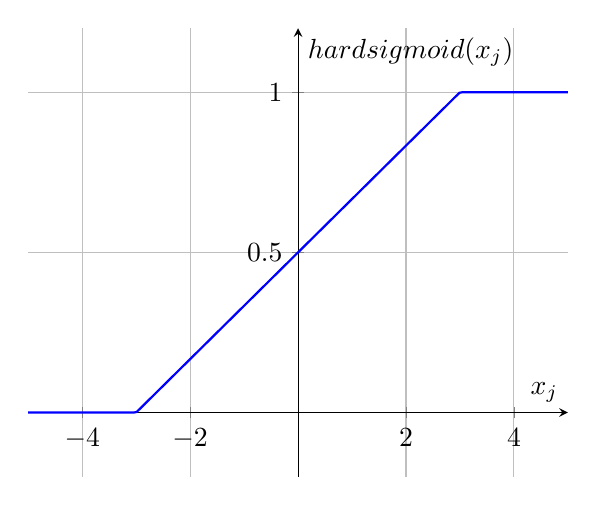
\begin{tikzpicture}
        \begin{axis}[
            xlabel={$x_j$},
            ylabel={$\text{hard sigmoid}(x_j)$},
            xmin=-5, xmax=5,
            ymin=-0.2, ymax=1.2,
            axis lines=middle,
            grid=major,
            domain=-5:5,
            samples=200, % More samples for a smoother piecewise look
            restrict y to domain*=-0.2:1.2 % Keep plot within y limits
        ]
        % Define the piecewise function using if-else logic for plotting
        \addplot[blue, thick] {
            (x < -3) * 0 +
            (x >= -3 && x <= 3) * (x/6 + 0.5) +
            (x > 3) * 1
        };
        \end{axis}
    \end{tikzpicture}
    \caption{Gráfico da função de ativação \textit{hard sigmoid}.}%
    \label{fig:hard-sigmoid}
    \fonte{O autor (2025).}
\end{figure}

\medskip
\begin{center}
 * * *
\end{center}
\medskip

\textbf{Características da Hard Sigmoid}
\vspace{1em}

\begin{itemize}
    \item \textbf{Continuidade, suavidade e diferenciabilidade:}
    \item \textbf{Não-linearidade:}
    \item \textbf{Piecewise-linear:}
\end{itemize}

\medskip
\begin{center}
 * * *
\end{center}
\medskip

Com relação a derivada da \textit{hard sigmoid}, para obtê-lá, deve-se derivar todas as três expressões construindo a sua derivada. Note que os pontos que as retas se tocam no gráfico da Figura~\ref{fig:hard-sigmoid} são pontos de descontinuidade, pois quando calculados os limites laterais nesses pontos eles serão diferentes. Isso faz com que essa função não possa ser derivada desses locais. Considerando isso, é possível expressar a derivada da \textit{hard sigmoid} com a Equação~\ref{eq:hard-sigmoid-derivada}.

\begin{equacaodestaque}{\textit{Hard Sigmoid} Derivada}
        \frac{d}{dx_j}[\mathcal{A}_{\text{Hard sigmoid}}](x_j) = \begin{cases} 0 & \text{se } x_j < -3 \\ 1/6 & \text{se } -3 < x_j < 3 \\ 0 & \text{se } x_j > 3 \end{cases}%
    \label{eq:hard-sigmoid-derivada}
\end{equacaodestaque}

Tendo a sua derivada, cabe também plotar o seu gráfico, o qual está presente na Figura~\ref{fig:hard-sigmoid-derivada}. Perceba mais uma vez que o gráfico não é suave que nem na sigmoide logística, perceba que ele também tenta imitar o comportamento do gráfico da derivada da sigmoide logística, neste caso, com retas ao invés de curvas. Mas ainda sim, essa derivada retorna valores muito pequenos, ficando susceptível ao problema do desaparecimento do gradiente assim como a sua variante \textit{soft}.

\begin{figure}[h!]
    \centering
    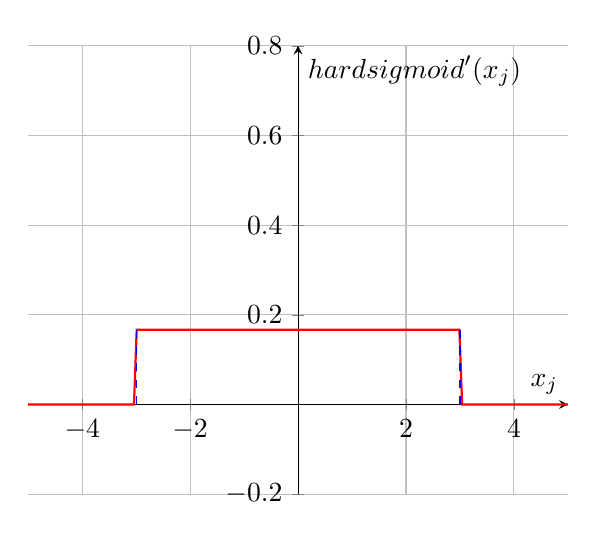
\begin{tikzpicture}
        \begin{axis}[
            xlabel={$x_j$},
            ylabel={$\text{hard sigmoid}'(x_j)$},
            xmin=-5, xmax=5,
            ymin=-0.2, ymax=0.8,
            axis lines=middle,
            grid=major,
            domain=-5:5,
            samples=200, % More samples to show step clearly
            restrict y to domain*=-0.2:0.8
        ]
        % Plot the derivative: 1/6 between -3 and 3, 0 otherwise
        \addplot[red, thick] {
            (x > -3 && x < 3) * (1/6)
        };
        % Add lines for the jumps (optional, but makes it clearer)
        \draw[dashed, blue] (axis cs:-3, 0) -- (axis cs:-3, 1/6);
        \draw[dashed, blue] (axis cs:3, 0) -- (axis cs:3, 1/6);
        \end{axis}
    \end{tikzpicture}
    \caption{Gráfico da derivada da função de ativação \textit{hard sigmoid}.}%
    \label{fig:hard-sigmoid-derivada}
    \fonte{O autor (2025).}
\end{figure}

Além disso, também existe a função \textit{hard tanh}, que apresenta a mesma proposta da \textit{hard sigmoid}, mas, nesse sentido, busca imitar o comportamento da função de ativação tangente hiperbólica. Para isso, ela segue uma ideia parecida com a da equação da \textit{hard sigmoid}, escrevendo a sua equação em forma de condicionais, mas ajustando os seus valores para corresponder ao funcionamento da tanh. Essa função está expressa na Equação~\ref{eq:hard-tanh}.

\begin{equacaodestaque}{\textit{Hard Tanh}}
        \mathcal{A}_{\text{Hard tanh}}(x_j) = \begin{cases} -1 & \text{se } x_j < -1 \\ x_j & \text{se } -1 \le x_j \le 1 \\ 1 & \text{se } x_j > 1 \end{cases}%
    \label{eq:hard-tanh}
\end{equacaodestaque}

Em que:

\begin{itemize}
    \item $x_j$ representa o valor da entrada da função de ativação
\end{itemize}

O seu gráfico também é parecido com o da \textit{hard sigmoid}. Como é possível vez na Figura~\ref{fig:hard-tanh}, ele é composto por três retas, sendo duas delas constantes e uma terceira sendo a função identidade. Note que ele também possui ``bicos'', o que o impede essa função de ser derivada nesses pontos, uma vez que ela não é contínua nessas regiões.

\begin{figure}[h!]
    \centering
    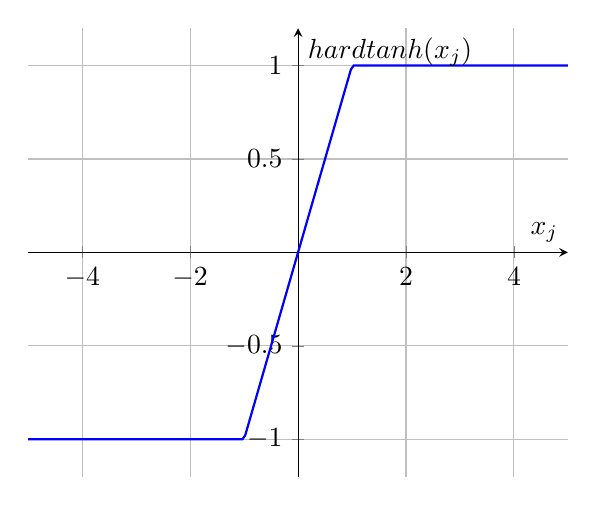
\begin{tikzpicture}
        \begin{axis}[
            xlabel={$x_j$},
            ylabel={$\text{hard tanh}(x_j)$},
            xmin=-5, xmax=5,
            ymin=-1.2, ymax=1.2,
            axis lines=middle,
            grid=major,
            domain=-5:5,
            samples=200, % More samples for clarity
            restrict y to domain*=-1.2:1.2 % Keep plot within y limits
        ]
        % Define the piecewise function for plotting
        \addplot[blue, thick] {
            (x < -1) * -1 +
            (x >= -1 && x <= 1) * x +
            (x > 1) * 1
        };
        \end{axis}
    \end{tikzpicture}
    \caption{Gráfico da função de ativação \textit{hard tanh}.}%
    \label{fig:hard-tanh}
    \fonte{O autor (2025).}
\end{figure}

\medskip
\begin{center}
 * * *
\end{center}
\medskip

\textbf{Características da Hard Tanh}
\vspace{1em}

\begin{itemize}
    \item \textbf{Continuidade, suavidade e diferenciabilidade:}
    \item \textbf{Não-linearidade:}
    \item \textbf{Piecewise-linear:}
\end{itemize}

\medskip
\begin{center}
 * * *
\end{center}
\medskip

Perceba também que o gráfico, bem como sua equação, é bem mais simples que a tangente hiperbólica tradicional, isso faz com que a \textit{hard tanh} seja uma função mais barata para ser empregada ao desenvolver um modelo de rede neural. Isso significa que ela pode ser uma função ideal para ser utilizada naqueles sistemas que possuem recursos limitados, como uma quantidade pequena de memória ram, ou seu a possibilidade de utilizar uma placa gráfica dedicada para o processamento dos dados. O mesmo vale para a \textit{hard sigmoid}.

Agora é possível também considerar também a derivada da \textit{hard tanh}, a qual é calculada de forma semelhante a da \textit{hard sigmoid}, derivando as três expressões de sua equação separadamente. Feito isso, a derivada da \textit{hard tanh} está expressa na Equação~\ref{eq:hard-tanh-derivada}.

\begin{equacaodestaque}{\textit{Hard Tanh} Derivada}
        \frac{d}{dx_j}[\mathcal{A}_{\text{Hard tanh}}](x_j) = \begin{cases} 0 & \text{se } x_j < -1 \\ 1 & \text{se } -1 < x_j < 1 \\ 0 & \text{se } x_j > 1 \end{cases}%
    \label{eq:hard-tanh-derivada}
\end{equacaodestaque}

Tendo a derivada, o próximo passo é plotar o seu gráfico, que pode ser visto na Figura~\ref{fig:hard-tanh-derivada}. Note mais uma vez que ele também tenta imitar o comportamento da derivada da tangente hiperbólica, porém, sendo composto por retas ao invés de uma curva suave. Novamente, é possível perceber que a \textit{hard tanh} também irá sofrer do problema do desaparecimento do gradiente, uma vez que retorna valores muito pequenos para a sua derivada.

\begin{figure}[h!]
    \centering
    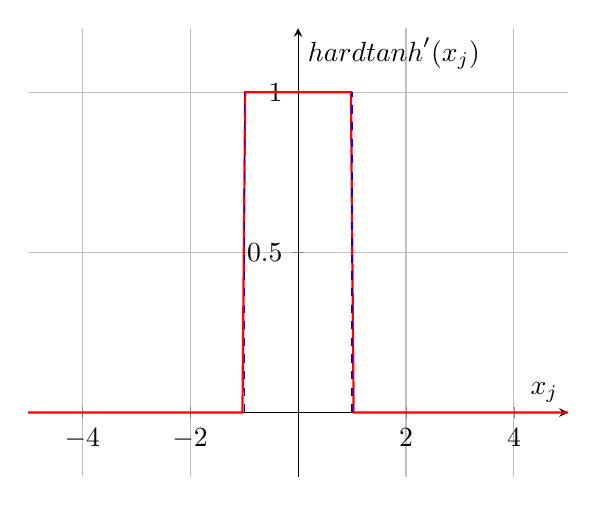
\begin{tikzpicture}
        \begin{axis}[
            xlabel={$x_j$},
            ylabel={$\text{hard tanh}'(x_j)$},
            xmin=-5, xmax=5,
            ymin=-0.2, ymax=1.2,
            axis lines=middle,
            grid=major,
            domain=-5:5,
            samples=200, % More samples to show step clearly
            restrict y to domain*=-0.2:1.2
        ]
        % Plot the derivative: 1 between -1 and 1, 0 otherwise
        \addplot[red, thick] {
            (x > -1 && x < 1) * 1
        };
        % Add lines for the jumps (optional, but makes it clearer)
        \draw[dashed, blue] (axis cs:-1, 0) -- (axis cs:-1, 1);
        \draw[dashed, blue] (axis cs:1, 0) -- (axis cs:1, 1);
        \end{axis}
    \end{tikzpicture}
    \caption{Gráfico da derivada da função de ativação \textit{hard-tanh}.}%
    \label{fig:hard-tanh-derivada}
    \fonte{O autor (2025).}
\end{figure}

\medskip
\begin{center}
 * * *
\end{center}
\medskip

\textbf{Algumas Aplicações das Funções Hard Sigmoid e Hard Tanh em Redes Neurais}%
\index{Aplicações práticas!Hard Tanh}%
\index{Aplicações práticas! Hard Sigmoid}
\vspace{1em}

\begin{itemize}
    \item \textbf{Aplicação 1 (Área):}
    \item \textbf{Aplicação 2 (Área):}
    \item \textbf{Aplicação 3 (Área):}
    \item \textbf{Aplicação 4 (Área):}
\end{itemize}

\medskip
\begin{center}
 * * *
\end{center}
\medskip

Conhecendo todas essas diferentes funções de ativação, é possível finalmente entender o que é o problema do desaparecimento de gradientes e como ele ocorre em uma rede neural, além de relacionar a atuação das funções sigmoidais com o aparecimento desse fenômeno. Para isso, é possível ver essas explicações na seção a seguir.

\section{O Desaparecimento de Gradientes}%
\index{Desaparecimento de gradientes}

Mesmo possuindo muitas propriedades atrativas para a utilização da familia sigmoidal em redes neurais, como a continuidade em todos os pontos e suavidade, além de que suas derivadas podem ser feitas com as próprias funções (no caso da sigmoide e da tangente hiperbólica), essa familia de funções trouxe um problema para os cientistas da época.

Como foi destacado ao discutir o gráfico das derivadas dessas funções, é possível notar que para valores extremos, seja eles positivos ou negativos, a derivada dessas funções fica bem próxima de zero. Isso significa que quando essas funções recebem como entrada um valor alto no \textit{forward pass}, na retropropagação, por pegarmos esse valor e calcularmos a derivada da função de ativação naquele ponto, irá retornar um valor baixo.

Para explicar melhor essa condição será utilizado um problema como base.

Como foi visto no capítulo anterior, o gradiente retropropagado para camadas anteriores de uma rede neural é proporcional a multiplicação da perda, com a derivada da função de ativação no ponto e o valor do resultado da camada anterior de neurônios. 

\[
    \delta^{(L)} = \left( \left( \textbf{W}^{(L+1)} \right)^T \delta^{(L+1)} \right)  \odot \mathcal{A}'(x^{(L)})
\]

Em que: 

\begin{itemize}
    \item $L$: Representa o índice de uma camada, podendo ser um valor entre $1$ (indicando que é uma camada de entrada) ou $n$ (indicando que é uma camada de saída);
    \item $\textbf{W}^{(L)}$: Representa a matriz dde pesos que conecta a camada $L - 1$ à camada $L$;
    \item $b^{(L)}$: Representa o vetor de viés da camada $L$;
    \item $x^{(L)}$: Representa o vetor de entradas totais para os neurônios da camada $L$ antes da ativação;
    \item $y^{(L)}$: Representa o vetor de saídas da camada $L$
    \item $\delta^{(L)}$: Representa o vetor do gradiente na camada $L$;
    \item $\mathcal{A}'(x^{(L)})$: Representa o vetor contendo a derivada da função de ativação para cada neurônio da camada $L$;
    \item $\odot$: O produto de Hadamard, que significa multiplicação elemento a elemento.
\end{itemize}

Considerando isso, imagine que temos uma rede composta por quatro camadas densas e cada camada tem apenas um neurônio com pesos iguais a 1. Dessa forma, é possível simplificar a fórmula vista para a Equação~\ref{eq:gradiente-retropropagado-simplificado}.

\begin{equation}
        \delta^{(L)} =  \delta^{(L+1)} \times \mathcal{A}'(x^{(L)})
        \label{eq:gradiente-retropropagado-simplificado}
\end{equation}

Considere também que as camadas da rede possuem a seguinte configuração:

\begin{itemize}
    \item Sigmoide da primeira camada: tem como resultado da derivada $\sigma'(x_j) = 0.2$
    \item Sigmoide da camada densa 2: tem como resultado da derivada $\sigma'(x_j) = 0.05$
    \item Sigmoide da camada densa 3: tem como resultado da derivada $\sigma'(x_j) = 0.1$
    \item Sigmoide da camada de saída: tem como resultado da derivada $\sigma'(x_j) = 0.08$
\end{itemize}

Além disso, você sabe também que o gradiente inicial na camada de saída está sendo de 1. Com isso é possível calcular o gradiente retropropagado para a primeira camada, começando pela terceira, já que já temos o valor do gradiente para a camada de saída, dessa forma temos que:

\[\begin{WithArrows}
    \delta^{(3)} & = \delta^{(4)} \times \sigma'(x^{(3)}) \Arrow{Subtituindo os valores} \\
    \delta^{(3)} & = 1 \times 0.1 = 0.1
\end{WithArrows}\]

Seguindo adiante, é possível fazer o mesmo procedimento para encontrar $\delta^{(2)}$ agora já tendo $\delta^{(3)}$, dessa forma:

\[\begin{WithArrows}
    \delta^{(2)} & = \delta^{(3)} \times \sigma'(x^{(2)}) \Arrow{Subtituindo os valores} \\
    \delta^{(2)} & = 0.1 \times 0.05 = 0.005
\end{WithArrows}\]

De forma semelhante, é finalmente possível encontrar o gradiente retropropagado para a primeira camada:

\[\begin{WithArrows}
    \delta^{(1)} & = \delta^{(2)} \times \sigma'(x^{(1)}) \Arrow{Subtituindo os valores} \\
    \delta^{(1)} & = 0.005 \times 0.2 = 0.001
\end{WithArrows}\]

Note que o gradiente que entrou ao ser calculado pela perda era de 1, no final da camada chegou apenas 0.001, ou seja, ele diminui mil vezes. Se considerarmos uma situação como esta, em que a derivada função de ativação irá retornar uma valor baixo, esse valor será multiplicado com os outros termos da expressão fazendo com que o valor total do gradiente retropropagado naquela camada seja baixo. Nós também vimos que redes em que é utilizada a retropropagação, cálculo do gradiente é utilizado como forma de fazer com que os pesos e vieses dos neurônios se atualizem e com isso a rede aprenda. E se os pesos são atualizados com uma variação muito pequena quando comparamos com seus valores anteriores, isso significa que essa rede estaria dando pequenos passos para encontrar a sua função. 

Ao passar valores muito extremos para uma função de ativação sigmoide, estamos prejudicando o aprendizado de uma rede neural, pois isso implica em derivadas com valores pequenos e consequentemente gradientes retropropagados pequenos. Agora imagine que em uma rede neural pode existir diversas camadas densas que usem a função sigmoide, se cada vez que o gradiente passar para a camada anterior ele diminuir, isso significa que na primeira camada, a última a ter seus pesos atualizados, o gradiente será tão pequeno que pode ser que não contribua para que a rede aprenda corretamente. É como se toda vez que passasse um valor muito extremo para a rede, o tamanho do passo que ela dá em direção a função procurada diminuísse. Assim, tem-se o problema do desaparecimento do gradiente.

\begin{definicaomoderna}{\textbf{Definição:}}
Quando o gradiente é muito pequeno em valor absoluto, ou até mesmo igual a zero, a atualização do gradiente apresenta quase nenhum impacto nos parâmetros de uma rede neural, fazendo com que não haja progresso nos parâmetros de aprendizado, dessa forma o \textbf{desaparecimento do gradiente} é quando esse fenômeno acontece repetidamente por várias pares de entrada e saída. \parencite{ActivationFunctionsLederer}.
\end{definicaomoderna}

Isso se torna um problema, pois, quando criamos uma rede neural, utilizamos as primeiras camadas para que elas sejam responsáveis por aprender características básicas/simples de uma determinada amostra de dados. Se o gradiente é próximo de zero, o calculo da atualização dos pesos e dos vises irá gerar valores muito próximos dos originais. Como esses valores não irão atualizar corretamente, a rede neural não irá aprender características básicas de um cenário.

Nesse sentido, o Capítulo~\ref{cap:ativacao-retificadoras} busca explicar as funções retificadoras, começando pela \textit{ReLU}, e como elas vieram como uma alternativa para contornar o \gls{vanishing-gradient-problem}. Contudo, elas também não foram perfeitas, e acabaram por introduzir os seus próprios problemas ao serem aplicadas em uma rede neural. Neste caso, um dos problemas que pode ocorrer ao se utilizar uma função retificadora é o problema da explosão do gradiente, e considerando a \textit{ReLU}, ela também pode causar um problema conhecido como \textit{ReLUs} agonizantes.

Assim, o último passo ao conhecer todas essas funções, é resumir o seu conteúdo para melhor entendimento. Este resumo pode ser visto na próxima seção.

\section{Comparativo: Funções Sigmoidais}%
\index{Comparativos!Funções sigmoidais}

Tendo visto diferentes funções de ativação sigmoidais, é possível compilá-las em na Tabela~\ref{tab:comparativo-funcoes-sigmoidais}, destacando as suas fórmulas, vantagens e desvantagens ao serem utilizadas em uma rede neural.

\begin{table}[htbp]
    \centering
    \begin{threeparttable}
        \caption{Comparativo das funções de ativação sigmoidais}%
        \label{tab:comparativo-funcoes-sigmoidais}
        \begin{tabularx}{\textwidth}{p{3.2cm} *{2}{>{\raggedright\arraybackslash}X}}
            \toprule
            \textbf{Função} & \textbf{Vantagem} & \textbf{Desvantagem} \\
            \midrule
            Sigmoide logística & Pode ser interpretada como uma probabilidade, podendo ser aplicada nas camadas de saída para classificação binária. & Não é centrada em zero, fazendo com que a convergência de modelos que usem essa função seja um pouco mais lenta. \\
            \addlinespace
            Tangente hiperbólica & Centrada em zero, garantindo uma convergência mais rápida de modelos que usem essa função. & Possui muitos exponenciais, sendo uma função ``cara'' em termos de custo computacional. \\
            \addlinespace
            \textit{Softsign} & É uma sigmoidal mais ``barata'' em termos de custo computacional, permitindo a criação de redes mais rápidas. & Sua derivada não pode ser escrita de forma recursiva. \\
            \addlinespace
            \textit{Hard Sigmoid} & É uma versão mais ``barata'' da sigmoide logística. & Não é uma função suave, possuindo ``quinas'', as quais impedem essa função de ser derivada nesses pontos. \\
            \addlinespace
            \textit{Hard Tanh} & É uma versão mais ``barata'' da tangente hiperbólica. & Assim como a \textit{hard sigmoid}, a \textit{hard tanh} apresenta ``quinas'', as quais impedem essa função de ser derivada nesses pontos. \\
        \end{tabularx}
        
        \begin{tablenotes}[para]
            \small
            \item[] Fonte: O autor (2025).
        \end{tablenotes}

    \end{threeparttable}
\end{table}

\medskip
\begin{center}
 * * *
\end{center}
\medskip

\textbf{Indo Além das Funções de Ativação Sigmoidais}
\medskip

Nesse capítulo foi visto um dos grandes grupos de função de ativação: as funções sigmoidais. Foi visto que elas estiveram presente em uma gama de redes neurais do século passado, fazendo parte da definição da retropropagação e também da rede de Elman, por exemplo. Contudo, a sua natureza saturante fazia com que a sua derivada atingisse valores muito pequenos, como 0.25. Isso atrapalhava a retropropagação do gradiente, que era constantemente multiplicado por escalares pequenos resultando no problema do desaparecimento do gradiente.

Esse problema impedia a criação de redes neurais muito profundas, pois quando mais camadas densas fossem adicionadas, maior era a chance de que seriam adicionadas como função de ativação uma função sigmoidal, aumentando ainda mais o risco de gerar problemas com o gradiente. isso foi um problema sério e que precisava de uma solução, e ela veio de uma forma bem simples e elegante, que foi com o uso da unidade linear retificadora, ou \textit{ReLU}. A \textit{ReLU} e a sua família de funções retificadoras é o tema central do capítulo que sucede este, o Capítulo~\ref{cap:ativacao-retificadoras}, ele segue a mesma estrutura deste capítulo, é apresentado o contexto em que essas funções surgiram e se popularizaram, bem como suas fórmulas e derivadas. Além disso, o Capítulo~\ref{cap:ativacao-retificadoras} também explica alguns problemas que essas funções acabaram causando com o gradiente na rede, sendo eles o \textit{dying ReLUs problem} e o problema do gradiente explosivo.

\medskip
\begin{center}
 * * *
\end{center}
\medskip